
\documentclass{Configuration_Files/PoliMi3i_thesis}

%------------------------------------------------------------------------------
%	REQUIRED PACKAGES AND  CONFIGURATIONS
%------------------------------------------------------------------------------

% CONFIGURATIONS
\usepackage{parskip} % For paragraph layout
\usepackage{setspace} % For using single or double spacing
\usepackage{emptypage} % To insert empty pages
\usepackage{multicol} % To write in multiple columns (executive summary)
\setlength\columnsep{15pt} % Column separation in executive summary
\setlength\parindent{0pt} % Indentation
\raggedbottom  

% PACKAGES FOR TITLES
\usepackage{titlesec}
% \titlespacing{\section}{left spacing}{before spacing}{after spacing}
\titlespacing{\section}{0pt}{3.3ex}{2ex}
\titlespacing{\subsection}{0pt}{3.3ex}{1.65ex}
\titlespacing{\subsubsection}{0pt}{3.3ex}{1ex}
\usepackage{color}

% PACKAGES FOR LANGUAGE AND FONT

\usepackage[utf8]{inputenc} % UTF8 encoding
\usepackage[T1]{fontenc} % Font encoding
\usepackage[11pt]{moresize} % Big fonts

% PACKAGES FOR IMAGES
\usepackage{graphicx}
\usepackage{transparent} % Enables transparent images
\usepackage{eso-pic} % For the background picture on the title page
\usepackage{subfig} % Numbered and caption subfigures using \subfloat.
\usepackage{tikz} % A package for high-quality hand-made figures.
\usetikzlibrary{}
\graphicspath{{./Images/}} % Directory of the images
\usepackage{caption} % Coloured captions
\usepackage{xcolor} % Coloured captions
\usepackage{amsthm,thmtools,xcolor} % Coloured "Theorem"
\usepackage{float}

% STANDARD MATH PACKAGES
\usepackage{amsmath}
\usepackage{amsthm}
\usepackage{amssymb}
\usepackage{amsfonts}
\usepackage{bm}
\usepackage[overload]{empheq} % For braced-style systems of equations.
\usepackage{fix-cm} % To override original LaTeX restrictions on sizes

% PACKAGES FOR TABLES
\usepackage{tabularx}
\usepackage{longtable} % Tables that can span several pages
\usepackage{colortbl}

% PACKAGES FOR ALGORITHMS (PSEUDO-CODE)
\usepackage{algorithm}
\usepackage{algorithmic}

% PACKAGES FOR REFERENCES & BIBLIOGRAPHY
\usepackage[colorlinks=true,linkcolor=black,anchorcolor=black,citecolor=black,filecolor=black,menucolor=black,runcolor=black,urlcolor=black]{hyperref} % Adds clickable links at references
\usepackage{cleveref}
\usepackage[square, numbers, sort&compress]{natbib} % Square brackets, citing references with numbers, citations sorted by appearance in the text and compressed
\bibliographystyle{abbrvnat} % You may use a different style adapted to your field

% OTHER PACKAGES
\usepackage{pdfpages} % To include a pdf file
\usepackage{afterpage}
\usepackage{lipsum} % DUMMY PACKAGE
\usepackage{fancyhdr} % For the headers
\fancyhf{}

% Input of configuration file. Do not change config.tex file unless you really know what you are doing. 
% Define blue color typical of polimi
\definecolor{bluepoli}{cmyk}{0.4,0.1,0,0.4}

% Custom theorem environments
\declaretheoremstyle[
  headfont=\color{bluepoli}\normalfont\bfseries,
  bodyfont=\color{black}\normalfont\itshape,
]{colored}

% Set-up caption colors
\captionsetup[figure]{labelfont={color=bluepoli}} % Set colour of the captions
\captionsetup[table]{labelfont={color=bluepoli}} % Set colour of the captions
\captionsetup[algorithm]{labelfont={color=bluepoli}} % Set colour of the captions

\theoremstyle{colored}
\newtheorem{theorem}{Theorem}[chapter]
\newtheorem{proposition}{Proposition}[chapter]

% Enhances the features of the standard "table" and "tabular" environments.
\newcommand\T{\rule{0pt}{2.6ex}}
\newcommand\B{\rule[-1.2ex]{0pt}{0pt}}

% Pseudo-code algorithm descriptions.
\newcounter{algsubstate}
\renewcommand{\thealgsubstate}{\alph{algsubstate}}
\newenvironment{algsubstates}
  {\setcounter{algsubstate}{0}%
   \renewcommand{\STATE}{%
     \stepcounter{algsubstate}%
     \Statex {\small\thealgsubstate:}\space}}
  {}

% New font size
\newcommand\numfontsize{\@setfontsize\Huge{200}{60}}

% Title format: chapter
\titleformat{\chapter}[hang]{
\fontsize{50}{20}\selectfont\bfseries\filright}{\textcolor{bluepoli} \thechapter\hsp\hspace{2mm}\textcolor{bluepoli}{|   }\hsp}{0pt}{\huge\bfseries \textcolor{bluepoli}
}

% Title format: section
\titleformat{\section}
{\color{bluepoli}\normalfont\Large\bfseries}
{\color{bluepoli}\thesection.}{1em}{}

% Title format: subsection
\titleformat{\subsection}
{\color{bluepoli}\normalfont\large\bfseries}
{\color{bluepoli}\thesubsection.}{1em}{}

% Title format: subsubsection
\titleformat{\subsubsection}
{\color{bluepoli}\normalfont\large\bfseries}
{\color{bluepoli}\thesubsubsection.}{1em}{}

% Shortening for setting no horizontal-spacing
\newcommand{\hsp}{\hspace{0pt}}

\makeatletter
% Renewcommand: cleardoublepage including the background pic
\renewcommand*\cleardoublepage{%
  \clearpage\if@twoside\ifodd\c@page\else
  \null
  \AddToShipoutPicture*{\BackgroundPic}
  \thispagestyle{empty}%
  \newpage
  \if@twocolumn\hbox{}\newpage\fi\fi\fi}
\makeatother

%For correctly numbering algorithms
\numberwithin{algorithm}{chapter}

%----------------------------------------------------------------------------
%	NEW COMMANDS DEFINED
%----------------------------------------------------------------------------

% EXAMPLES OF NEW COMMANDS
\newcommand{\bea}{\begin{eqnarray}} % Shortcut for equation arrays
\newcommand{\eea}{\end{eqnarray}}
\newcommand{\e}[1]{\times 10^{#1}}  % Powers of 10 notation

%----------------------------------------------------------------------------
%	ADD YOUR PACKAGES (be careful of package interaction)
%----------------------------------------------------------------------------
\definecolor{codegreen}{rgb}{0,0.6,0}
\definecolor{codegray}{rgb}{0.5,0.5,0.5}
\definecolor{codepurple}{rgb}{0.58,0,0.82}
\definecolor{backcolour}{rgb}{0.95,0.95,0.92}
\usepackage{color}   %May be necessary if you want to color links
\usepackage{hyperref}
\usepackage{graphicx}
\usepackage[utf8]{inputenc}
\usepackage{listings}
\usepackage{xcolor}
\hypersetup{
	colorlinks=true, %set true if you want colored links
	linktoc=all,     %set to all if you want both sections and subsections linked
	linkcolor=black,  %choose some color if you want links to stand out
	urlcolor=blue,
}
\lstdefinestyle{mystyle}{
	backgroundcolor=\color{backcolour},
	commentstyle=\color{codegreen},
	keywordstyle=\color{magenta},
	numberstyle=\tiny\color{codegray},
	stringstyle=\color{codepurple},
	basicstyle=\ttfamily\footnotesize,
	breakatwhitespace=false,
	breaklines=true,
	captionpos=b,
	keepspaces=true,
	numbers=left,
	numbersep=5pt,
	showspaces=false,
	showstringspaces=false,
	showtabs=false,
	tabsize=2
}

\lstset{style=mystyle}


%----------------------------------------------------------------------------
%	BEGIN OF YOUR DOCUMENT
%----------------------------------------------------------------------------

\begin{document}

\fancypagestyle{plain}{%
\fancyhf{} % Clear all header and footer fields
\fancyhead[RO,RE]{\thepage} %RO=right odd, RE=right even
\renewcommand{\headrulewidth}{0pt}
\renewcommand{\footrulewidth}{0pt}}

%----------------------------------------------------------------------------
%	TITLE PAGE
%----------------------------------------------------------------------------

\pagestyle{empty} % No page numbers
\frontmatter % Use roman page numbering style (i, ii, iii, iv...) for the preamble pages

\puttitle{
	title=Systems and Methods for Big and Unstructured Data Project,
	name1=Gabriele Ginestroni, % Author Name and Surname
	name2=Giacomo Gumiero,
	name3=Lorenzo Iovine,
	name4=Nicola Landini,
	name5=Francesco Leone,
	academicyear=2022-2023,
	groupnumber=10
} % These info will be put into your Title page

\startpreamble
\setcounter{page}{1} % Set page counter to 1

%----------------------------------------------------------------------------
%	LIST OF CONTENTS/FIGURES/TABLES/SYMBOLS
%----------------------------------------------------------------------------

% TABLE OF CONTENTS
\thispagestyle{empty}
\tableofcontents % Table of contents
\thispagestyle{empty}
\cleardoublepage

\addtocontents{toc}{\vspace{2em}} % Add a gap in the Contents, for aesthetics
\mainmatter % Begin numeric (1,2,3...) page numbering

\chapter{Introduction}
\label{ch:introduction}
In this chapter will be presented the problem specification and the hypothesis under which the database is implemented.

\section{Problem Specification}
This project aims to build a documental database that handles scientific articles contained in the DBLP bibliography.
The focus is on creating a database which allows efficient information retrieval of the articles, including
their chapters and images.
The main collections analyzed in the project are \emph{Authors} and \emph{Publication} with all their attributes and related
objects like: \emph{chapters, biographies} and \emph{images}.

\section{Assumptions}
\label{sec:assumptions}
\begin{enumerate}
\item Articles can be published on a single venue
\item There is no distinction between different types of Publication
\item An author can't work for more than one organization for the same Publication
\item A chapter can contain subsections and these will be considered chapters as well
\end{enumerate}

\chapter{ER Diagram}
\label{ch:erd}
\begin{figure}[H]
	\centering
	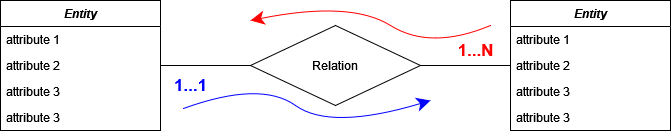
\includegraphics[width=0.6\textwidth]{legendaER.png}
	\caption{ER Diagram Organization}
	\label{fig:erleg}
\end{figure}
\bigskip
\begin{figure}[H]
	\centering
	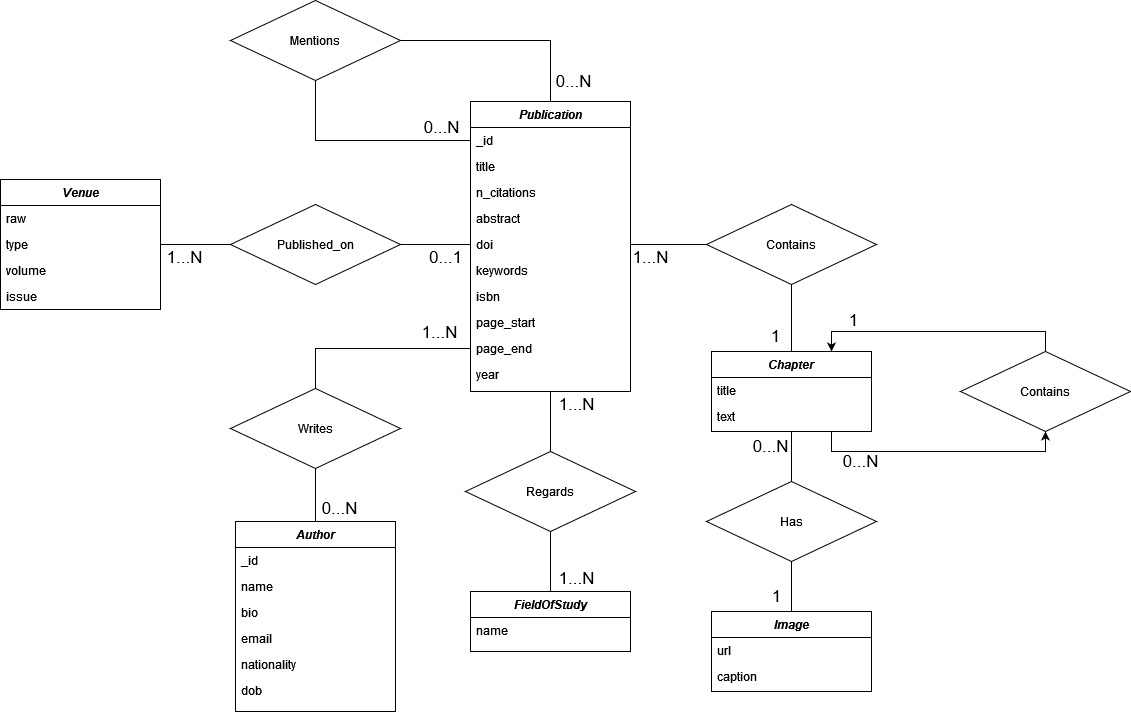
\includegraphics[width=1\textwidth]{ERDocDb.png}
	\caption{ER Diagram}
	\label{fig:er}
\end{figure}
\newpage

The Entity-Relationship model contains 6 main entities, that are related to each other through various relationships:
\begin{itemize}
	\item \textbf{Publication:} represents all the scientific articles. Its attributes are: \emph{\_id, title, n\_citations,
		abstract, doi, keywords, isbn, page\_start, page\_end, year} and its organization will be presented later
	\item \textbf{Author:} it is the one who contributed to a publication. Its attributes are: \emph{\_id, name, bio,
		email, nationality, dob (date of birth)}
	\item \textbf{Venue:} it is where a publication is published or presented. Its attributes are: \emph{raw, type,
		volume, issue}
	\item \textbf{FieldOfStudy:} this entity represents the subjects of the publication and its attribute is \emph{name}
	\item \textbf{Chapter:} it represents the chapter of a scientific articles. Its attributes are \emph{title, text}
	\item \textbf{Image:} it represents the image contained in a specific chapter of the publication. Its attributes are
		\emph{url, caption}
\end{itemize}

The ER diagram designed contains also the following relationships:
\begin{itemize}
	\item \textbf{Mentions:} is the relationship between a \emph{publication} and another \emph{publication} cited by the first one
	\item \textbf{Published\_on:} is the relationship between a \emph{publication} and its \emph{venue}
	\item \textbf{Writes:} is the relationship between \emph{author} and \emph{publication} which features the affiliation property.
		We decided to design it with \verb |affiliation| as an attribute of the relationship, due to the fact that it belongs
		only to a pair of \emph{author} and \emph{publication} and it represents the institute where the author worked for the publication
	\item \textbf{Regards:} is the relationship between a \emph{publication} and its \emph{fields of study}
	\item \textbf{Contains:} is the relationship between \emph{publication} and its \emph{chapters} 
	\item \textbf{Composed\_by:} is the relationship between two \emph{chapters}. It represents the relationship created
		between a chapter and its sections, between a section and its subsection and so on. Note that we used a directed
		arrow in order to indicate that a section belongs only to a chapter, but a chapter could own more than one section.
	\item \textbf{Has:} is the relationship between \emph{chapter} and its \emph{images}
\end{itemize}


\chapter{Document Structure}
\label{ch:document_structure}
In this section we will describe the structure of our database. We decided to split our dataset in two collections:
\emph{authors} and \emph{articles}. The reason behind this choice was to increase the performance and to reduce the
spatial complexity. For example if we need to modify the email of an author we just have to change the field in the
\emph{author} collection. Whereas, if we just kept one collection, very expensive update query would have been needed
(change the modified field in each author's sub-document of the entire article collection).\newline

Furthermore, to avoid redundancies we used manual references to bind the two collections.\newline

In order to show the number of \emph{Authors} and \emph{Articles} in our collections, we performed the two following queries:
\begin{figure}[H]
\centering
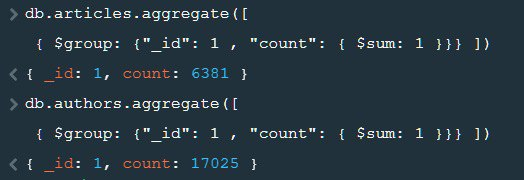
\includegraphics[width=0.7\textwidth]{instancenumber.jpg}
\label{fig:instances}
\end{figure}


\section{Data Preprocessing}
Starting from the database sample used for the Neo4j part some operations were performed to add the required fields and
to exploit better mongoDB functionalities. \newline
Missing \verb |isbn|, \verb |page_start|, \verb |page_end| attributes were added with random generations.\newline
Most important, chapters were added from the original paper pdf when available, and parsing was performed by using PHP
Library Smalot PDFParser. This library only parses the full text of the papers so the text was then divided into chapters
using chapter titles as a reference to split, thus it was possible to obtain the 2 attributes' title and text for each
chapter (for the \verb |text| field, only 10 rows were taken into consideration). A total of 170 pdfs were parsed and that
was also used as a pool to pick random chapters for papers that could not be parsed because their pdfs were not available
as a free copy on aminers' site.\newline
To add images and captions, a dataset of films and their covers from tmdb was used, for every chapter a random number of
images links were added combined with movie titles used as a caption.\newline
The advantage of aminers' dataset was the built-in \verb |_id| attribute for articles and authors and also the existence of an
array of references with the list of the referenced \verb |_id| inside every article tuple.\newline
To better exploit this opportunity we believe it was handy to have the 2 collections of articles and authors, so we
performed \verb |JSON| parsing of the dump to generate 2 new \verb |JSON| files:
\begin{itemize}
	\item one that contains the articles, with an array of authors that has inside the references to their \verb |_id| objectId
	\item the other contains the authors with an array of articles that has inside the references to their \verb |_id| objectId.
\end{itemize}
In the authors' collection the bio attribute was randomly generated only when not available, while \verb |email|, \verb |nationality| and
\verb |dob| attributes were 100\% randomly generated, especially:
\begin{itemize}
	\item \textbf{email:} was generated by concatenating Name.Surname with a pool of most famous mail servers(gmail.com, yahoo.com...)
	\item \textbf{nationality:} was generated by picking randomly from a pool of ~20 nation code
	\item \textbf{dob - date of birth:} was generated randomly from 1940 to 1992, so it may be possible that some inconsistencies are
		present (e.g. author that published before having 20 years old or even before being born)
\end{itemize}

\newpage
\section{Article structure}
In the following \verb |JSON| file we can see how the \emph{Article} is structured in our dataset.\newline
\textbf{Note:} in some fields we decided not to insert all the content only for ease of read reasons.\newline
\textbf{Note:} in \verb |venue|, fields \verb |issue|, \verb |volume| and \verb |publisher| are missing because they are empty in this example.
\begin{lstlisting}
{
"_id": {
	"$oid": "53e99f86b7602d9702859fdf"
},
"title": "Locality Sensitive Outlier Detection: A ranking driven approach",
"authors": [
	{
	"id": {
		"$oid": "542a4c9fdabfae61d496694e"
	},
	"org": "Computer Science and Engineering Department, OhioSU, USA"
	},
	{
	"id": {
		"$oid": "53f48bc5dabfaea7cd1cce1d"
	},
	"org": "Computer Science and Engineering Department, OhioSU, USA"
	},
	{
	"id": {
		"$oid": "53f44b6fdabfaec09f1dd00d"
	},
	"org": "Computer Science and Engineering Department, OhioSU, USA"
	}
],
"n_citation": 60,
"abstract": "Outlier detection is fundamental to a variety of database and...",
"doi": "10.1109/ICDE.2011.5767852",
"keywords": [
	"database point",
	"ranking scheme",
	"geometric approach",
	...
],
"isbn": "978-1-4244-8958-9",
"page_start": "410",
"page_end": "421",
"year": 2011,
"fos": [
	"Locality-sensitive hashing",
	"Anomaly detection",
	"Machine learning",
	...
],
"venue": {
	"raw": "ICDE",
	"type": 0,
},
"chapters": [
	{
	"title": "1. Introduction",
	"text": "Open Computing Language (OpenCL)[3] is a unified programming...",
	"images": [
		{
		"caption": "Giraffada",
		"link": "https://image.tmdb.org/t/p/w600_and_h900_bestv2/....jpg"
		},
		{
		"caption": "A Certain Magical Index: The Miracle Of Endymion",
		"link": "https://image.tmdb.org/t/p/w600_and_h900_bestv2/....jpg"
		},
		{
		"caption": "Ready To Rumble",
		"link": "https://image.tmdb.org/t/p/w600_and_h900_bestv2/....jpg"
		},
		{
		"caption": "Raw Force",
		"link": "https://image.tmdb.org/t/p/w600_and_h900_bestv2/....jpg"
		},
		{
		"caption": "The Departed",
		"link": "https://image.tmdb.org/t/p/w600_and_h900_bestv2/....jpg"
		},
		{
		"caption": "Repeaters",
		"link": "https://image.tmdb.org/t/p/w600_and_h900_bestv2/....jpg"
		}
	]
	},
	{
	"title": "2. The OpenCL Framework",
	"text": "21 Organization of Our Runtime\nThe target cluster...",
	"images": [
		{
		"caption": "The King Of New York",
		"link": "https://image.tmdb.org/t/p/w600_and_h900_bestv2/....jpg"
		},
		{
		"caption": "The Ghost Who Walks",
		"link": "https://image.tmdb.org/t/p/w600_and_h900_bestv2/....jpg"
		},
		{
		"caption": "Fighter In The Wind",
		"link": "https://image.tmdb.org/t/p/w600_and_h900_bestv2/....jpg"
		},
		{
		"caption": "Wake Up",
		"link": "https://image.tmdb.org/t/p/w600_and_h900_bestv2/....jpg"
		},
		{
		"caption": "Infierno Blanco",
		"link": "https://image.tmdb.org/t/p/w600_and_h900_bestv2/....jpg"
		},
		{
		"caption": "Bajo El Mismo Techo",
		"link": "https://image.tmdb.org/t/p/w600_and_h900_bestv2/....jpg"
		},
		{
		"caption": "Le Dernier Samaritain",
		"link": "https://image.tmdb.org/t/p/w600_and_h900_bestv2/....jpg"
		}
	]
	},
	{
	"title": "3. Evaluation",
	"text": "We have implemented the OpenCL runtime and...",
	"images": [
		{
		"caption": "L'hotel Degli Amori Smarriti",
		"link": "https://image.tmdb.org/t/p/w600_and_h900_bestv2/....jpg"
		},
		{
		"caption": "Bit",
		"link": "https://image.tmdb.org/t/p/w600_and_h900_bestv2/....jpg"
		},
		{
		"caption": "Dead Silence",
		"link": "https://image.tmdb.org/t/p/w600_and_h900_bestv2/....jpg"
		},
		{
		"caption": "Amenazados",
		"link": "https://image.tmdb.org/t/p/w600_and_h900_bestv2/....jpg"
		}
	]
	},
	{
	"title": "4. Conclusions",
	"text": "We introduce the design and implementation of...",
	"images": [
		{
		"caption": "Eddie The Eagle",
		"link": "https://image.tmdb.org/t/p/w600_and_h900_bestv2/....jpg"
		},
		{
		"caption": "Gorenos",
		"link": "https://image.tmdb.org/t/p/w600_and_h900_bestv2/....jpg"
		},
		{
		"caption": "Pinocchio",
		"link": "https://image.tmdb.org/t/p/w600_and_h900_bestv2/....jpg"
		},
		{
		"caption": "Le Grand Bazar",
		"link": "https://image.tmdb.org/t/p/w600_and_h900_bestv2/....jpg"
		},
		{
		"caption": "Gangsters",
		"link": "https://image.tmdb.org/t/p/w600_and_h900_bestv2/....jpg"
		},
		{
		"caption": "Kodachrome",
		"link": "https://image.tmdb.org/t/p/w600_and_h900_bestv2/....jpg"
		}
	]
	}
],
"references": [
	{
		"$oid": "53e99fddb7602d97028b7e65"
	}
]
}
\end{lstlisting}

\section{Author structure}
In the following \verb |JSON| file we can see how the \emph{Author} is structured in our dataset.\newline
\textbf{Note:} in some fields we decided not to insert all the content only for ease of read reasons.
\begin{lstlisting}
{
"_id": {
	"$oid": "53f45775dabfaee4dc8162e6"
},
"name": "Guillermo Jorge-Botana",
"articles": [
	{
	"$oid": "53e99f86b7602d970285a187"
	}
],
"orcid": "0000-0001-5879-6783",
"bio": "Qing-Long Han received the B.Sc. degree in mathematics from the...",
"email": "Guillermo.Jorge-Botana@yahoo.com",
"nationality": "de",
"dob": 1974-09-14T00:00:00.000+00:00
}
\end{lstlisting}

\newpage
\section{Attributes Description}
In this section we will present all the attributes contained in our filtered dataset.

\subsection{Article}
Publication represent the central concept of the system and contains:
\begin{itemize}
\item \textbf{\_id} is an ObjectId that identifies a publication.
\item \textbf{title} represents the title of the publication.
\item \textbf{authors} is an array of subdocuments that contains: ObjectId of the authors of the article and the \verb |org|
	field which represent the affiliation.
\item \textbf{n\_citation} is the number of times that the publication has been mentioned.
\item \textbf{abstract} is a string containing a brief summary of the contents of the paper.
\item \textbf{doi} Digital Object Identifier is a persistent and standardized identifier.
\item \textbf{keywords} is an array containing keywords of the publication.
\item \textbf{isbn} is an identification code of the venue of the publication.
\item \textbf{page\_start} defines the starting page of the publication.
\item \textbf{page\_end} defines the last page of the publication.
\item \textbf{year} represents the year of publication.
\item \textbf{fos} is an array containing the fields of study of the publication.
\item \textbf{venue} is a sub-document that represents where a publication is published or presented. This field contains:
				\begin{itemize}
					\item \textbf{raw} is the name or the abbreviation of the venue (regardless the year, issue or volume) in which the
						publication was presented.
					\item \textbf{type} indicates the type of the publication.
					\item \textbf{volume} is the volume of the venue in which the article has been published.
					\item \textbf{issue} refers to how many times a periodical has been published during that year.
					\item \textbf{publisher} is the name of the publisher of the article.
				\end{itemize}
\item \textbf{chapters} is an array of sub-documents containing containing \verb |title| (title of the chapter), \verb |text| (the content),
	 \verb |sections| (that has the same structure of a chapter). They also contains \verb |images| composed by:
				\begin{itemize}
					\item \textbf{caption} the caption of the image.
					\item \textbf{link} the link to the image.
				\end{itemize}
\item \textbf{references} set of ObjectIds of the referenced articles.
\end{itemize}
\bigskip

\subsection{Author}
The dataset provides the following author fields:
\begin{itemize}
\item \textbf{\_id} is an ObjectId that identifies an author.
\item \textbf{name} is the name of the author.
\item \textbf{articles} is a set of articles identifier of the publications of the author.
\item \textbf{orcid} Open Researcher and Contributor ID is a unique identifier for authors of scientific articles.
\item \textbf{bio} is a string that describes the author.
\item \textbf{email} is the email address of the author.
\item \textbf{nationality} is the nationality of the author.
\item \textbf{dob} is the birth date of the author.
\end{itemize}


\chapter{Commands and Queries}
\label{ch:ceq}
\section{Commands}
We have identified the following \verb |INSERT| and \verb |UPDATE| commands to show the system basic functionalities.

\subsection{Insert a publication in the system}
\label{pub_insert}
Assuming it is not present in the dataset, we inserted a new document that is a new instance of \emph{Publication}.
In order to do that we instantiated 5 different variables: \verb |article_id| that generates an ObjectId representing
the id of the article we're creating; \verb |article_ref1| and \verb |article_ref2| that are the ids of two scientific
articles cited by this publication; \verb |author1_id| and \verb |author2_id| that are the ids of the authors.\newline
\textbf{Note:} \verb |isbn| field is missing \newline
\textbf{Note:} \verb |type| = 1 represents a \emph{Journal} \newline
\textbf{Note:} \verb |issue| field is missing
\begin{lstlisting}
article_id = ObjectId()
article_ref1 = ObjectId("53e99fe4b7602d97028bf743")
article_ref2 = ObjectId("53e99fddb7602d97028bc085")
author1_id = ObjectId()
author2_id = ObjectId()

db.articles.insertOne({
	_id: article_id,
	title: "An extensive study of C-SMOTE, a Continuous Synthetic Minority Oversampling Technique for Evolving Data Streams",
	authors:
	[
		{id:author1_id, org:"Politecnico di Milano"},
		{id:author2_id, org:"Politecnico di Milano"}
	],
	n_citation: 3,
	abstract: "Streaming Machine Learning (SML) studies algorithms that update their models, given an unbounded and often non-stationary flow of data performing a single pass. Online class imbalance learning is a branch of SML that combines the challenges of both class imbalance and concept drift. In this paper, we investigate the binary classification problem by rebalancing an imbalanced stream of data in the presence of concept drift, accessing one sample at a time.",
	doi: "10.1016/j.eswa.2022.116630",
	keywords: ["Evolving Data Stream","Streaming","Concept drift","Balancing"],
	page_start: 39,
	page_end: 46,
	year: 2022,
	fos: ["Computer Science","Stream Reasoning","Big Data"],
	venue: {
		raw: "ESA",
		type: 1,
		volume: 196,
		publisher: "Elsevier"
	},
	chapters:
	[
		{
		title:"1. Introduction",
		text:"Nowadays, data abound as a multitude of smart devices, such as smartphones, wearables, computers, and Internet of Things (IoT) sensors produce massive, continuous, and unbounded flows of data, namely data streams. This poses several challenges to Machine Learning (ML)."
		},

		{
		title:"2. Background",
		text:"This section is divided into three parts describing the different concept drift types and characteristics, the evaluation metrics, and the most common approaches to use in class imbalance.",
		subsection: [
			{
			title:"2.1. Concept drift in evolving data streams",
			text:"In this part, we introduce the concept drift phenomenon explaining why and how it happens. We explain all its different types, forms, and possible speeds of occurrence.",
			subsubsection: [
				{
				title:"2.1.1. Concept drift types",
				text:"Since the generating function is unknown, concept drift is unpredictable. In the batch settings, with all the data available, it is simple to check	and detect if a dataset is not stationary.",
				images:
					[
						{
						caption:"Fig.1 Representation of the three different types of concept drift",
						url:"https://ars.els-cdn.com/content/image/1-s2.0-S0957417422001208-gr1.jpg"
						}
					]
				}
			]
			}
		]
		},

		{
		title:"3. C-SMOTE",
		text:"This section recalls the description of C-SMOTE, inspired by the Smote technique, originally presented in Bernardo, Gomes et al. (2020). C-SMOTE is designed to rebalance an imbalanced data stream, and it can be pipelined with any SML- model. C-SMOTE stands for Continuous-Smote, meaning that the new Smote version is applied continuously.",
		images:[
			{
			caption:"Fig. 2. Architecture of C-SMOTE meta-strategy pipelined with an Online Learner.",
			url: "https://ars.els-cdn.com/content/image/1-s2.0-S0957417422001208-gr5.jpg"
			}
		],
		subsection:[
			{
			title:"3.1. Artificial data streams",
			text: "To synthetically reproduce the different types of concept drifts shown in Section 2.1, we choose two of the most commonly used artificial data generators: SINE1 (Gama et al., 2004) and SEA (Street & Kim, 2001)."
			}
		]

		}
		],
	references: [
		article_ref1,
		article_ref2
	]

})
\end{lstlisting}


\subsection{Insert an author in the system}
Assuming he is not present in the dataset, we used \verb |insertOne| to create a new instance of \emph{Author}.\newline
\textbf{Note:} \verb |author1_id| and \verb|article_id|, refers to the variables instantiated in the previous
command (Section: ~\ref{pub_insert})
\begin{lstlisting}
db.authors.insertOne({
	_id: author1_id,
	name: "Emanuele Della Valle",
	orcid: "0000-0002-5176-5885",
	articles:[
		article_id
	],
	bio:"Emanuele Della Valle holds a PhD in Computer Science from the Vrije Universiteit Amsterdam and a Master degree in Computer Science and Engineering from Politecnico di Milano. He is associate professor at the Department of Electronics, Information and Bioengineering of the Politecnico di Milano.",
	email:"emanuele.dellavalle@gmail.com",
	nationality:"it",
	dob:ISODate("1975-03-07T00:00:00.000Z")
})
\end{lstlisting}

\subsection{Update the number of citations of referenced publications}
With the following snippet of code is possible to increment the \verb |n_citations| field of the \emph{Publications}
referenced by the article created in section ~\ref{pub_insert}.\newline
\textbf{Note:} in this command we used \verb |updateMany| in order to update both the referenced publications; \verb |update|
wasn't enough because only one of the two matching document would have been updated\\
\begin{lstlisting}
db.articles.updateMany(
	{ $or:[{_id:{$eq:ObjectId("53e99fe4b7602d97028bf743")}}, {_id:{$eq:ObjectId("53e99fddb7602d97028bc085")}}]},
	{ $inc: { n_citation: 1} }
)
\end{lstlisting}

\subsection{Modification of the biography of an author}
This command allows to access \emph{Authors} by field \verb |name| in order to append a string to field \verb |bio|
\begin{lstlisting}
db.authors.updateMany(
	{name: "Emanuele Della Valle"},
	[{ $set: { bio: { $concat: [ "$bio", "He recently become full professot at ETH Zurich." ] } } }]
)
\end{lstlisting}

\subsection{Add a publication to its author}
This command allows to add the new publication (\emph{Publication} creation presented in section ~\ref{pub_insert}), to
one of its \emph{Authors}. \newline
\textbf{Note:} we assumed \verb |newArticleId| as the identifier of the new publication and that \verb |author1_id|
refers to the variable instantiated in section ~\ref{pub_insert}
\begin{lstlisting}
newArticleId = ObjectId()

db.authors.updateOne(
	{ _id:author1_id },
	{ $push:{articles:newArticleId}}
)
\end{lstlisting}


\newpage
\section{Queries}
We have identified the following queries in order to show the system's basic functionalities.\newline
For ease of read reasons, we decided to show results obtained using \verb |project| operator, and, in some cases,
we showed only some of the results.

\subsection{Query 1}
This query returns one publication written after 2013 whose \verb |FieldOfStudy(fos)| contains \emph{'Machine learning'}.
\begin{lstlisting}
db.articles.findOne({
	"$and": [{year: {$gte:2013}}, {"fos":"Machine learning"}]
})
\end{lstlisting}
\begin{figure}[H]
\centering
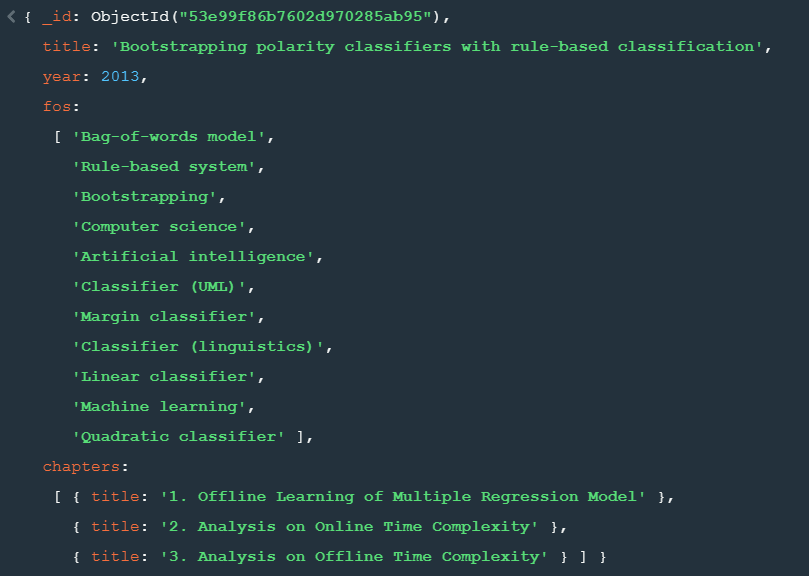
\includegraphics[width=1\textwidth]{query/mongo_q1.PNG}
\caption{Projection on title, fos, year, chapters.title}
\label{fig:query1}
\end{figure}

\newpage
\subsection{Query 2}
This query returns all the Italian authors born after 1960.
\begin{lstlisting}
db.authors.find({
	$and:[{nationality:'it'},{dob:{$gte:ISODate("1960-01-01")}}]
})
\end{lstlisting}
\begin{figure}[H]
\centering
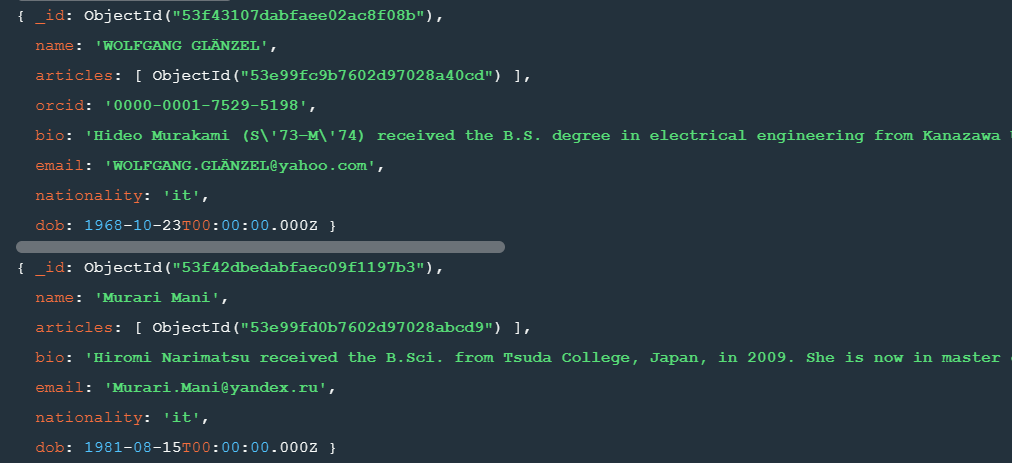
\includegraphics[width=1\textwidth]{query/mongo_q2.PNG}
\label{fig:query2}
\end{figure}

\subsection{Query 3}
This query returns ten of the articles published by \emph{'Elsevier'} after 2009.\newline
\textbf{Description:} this query perform a filtering over the year attribute of the article and on the publisher
field of the venue sub-document.
\begin{lstlisting}
db.articles.find({
	$and:[{"venue.publisher":'Elsevier'},{year:{$gte:2009}}]
}).limit(10)
\end{lstlisting}
\begin{figure}[H]
\centering
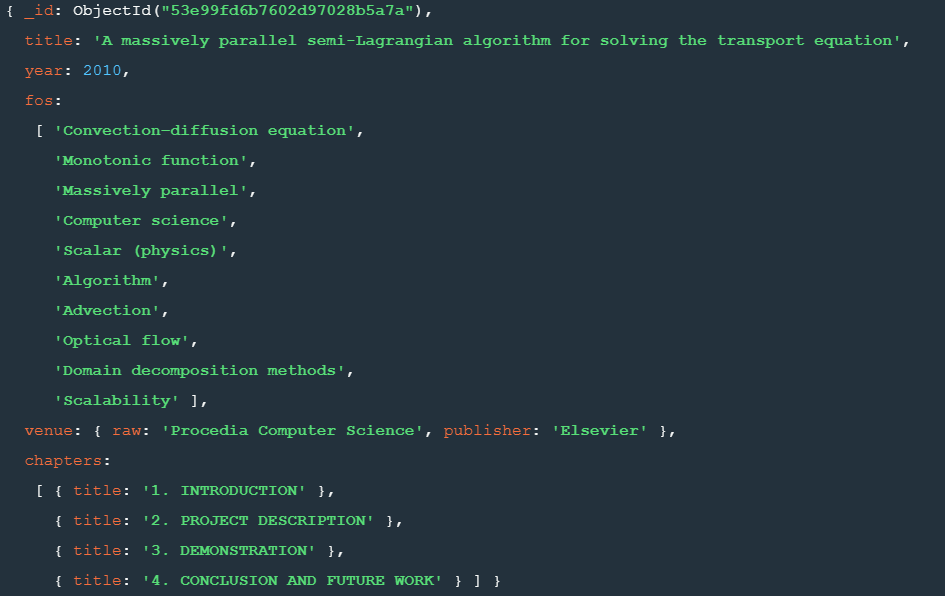
\includegraphics[width=0.85\textwidth]{query/mongo_q3.PNG}
\caption{Projection on title, fos, year, chapters.title, venue.raw, venue.publisher}
\label{fig:query3}
\end{figure}

\subsection{Query 4}
This query returns the top three years sorted by number of publications.\newline
\textbf{Description:} the query computes the count by aggregating with respect to the year field. Then groups
are sorted by descending order and only the top 3 are kept.
\begin{lstlisting}
db.articles.aggregate([
	{"$group" : {_id:"$year", count:{$sum:1}}},
	{"$sort": {count:-1}},
	{"$limit": 3}
]);
\end{lstlisting}
\begin{figure}[H]
\centering
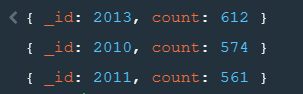
\includegraphics[width=0.6\textwidth]{query/mongo_q4.PNG}
\label{fig:query4}
\end{figure}

\subsection{Query 5}
This query finds all the articles with at least one Stanford affiliation and regarding \emph{'Machine learning'} field
of study. \newline
\textbf{Description:} this query perform a filtering over the fos attribute of the article and on the org field of the
authors array of sub-documents.
\begin{lstlisting}
db.articles.aggregate([
	{$match: {"authors.org":{$regex: "Stanford"}}},
	{$match: {"fos":"Machine learning"}}
])
\end{lstlisting}
\begin{figure}[H]
\centering
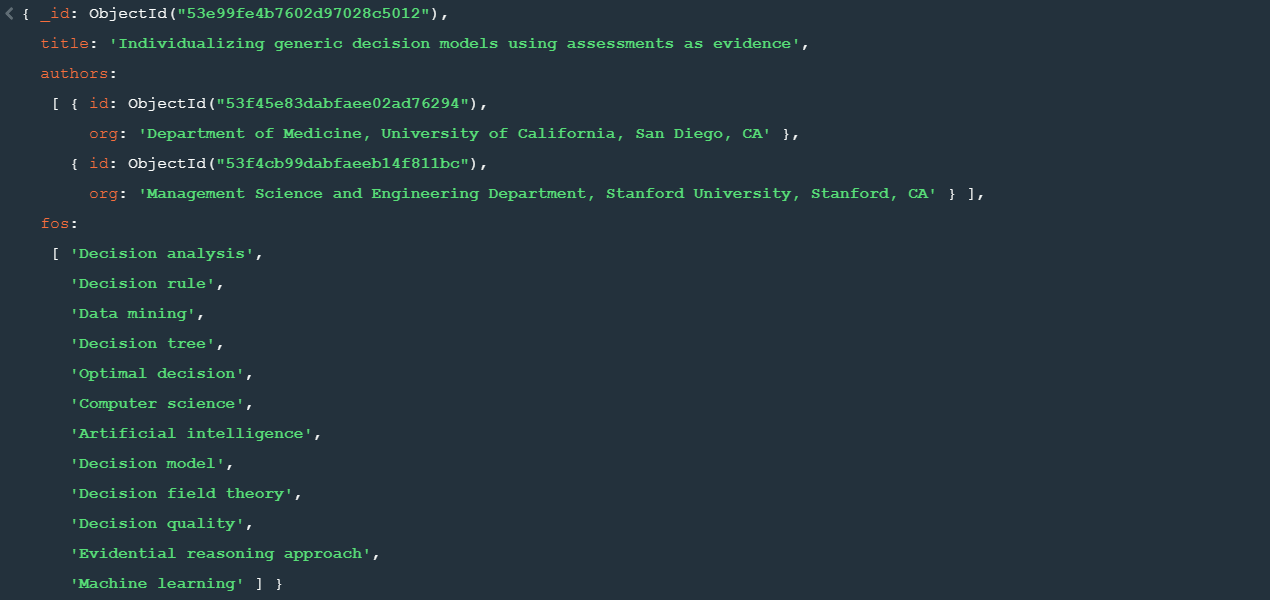
\includegraphics[width=1\textwidth]{query/mongo_q5.PNG}
\caption{Projection on authors, fos and title}
\label{fig:query5}
\end{figure}

\subsection{Query 6}
This query returns the top three years sorted by number of distinct authors.\newline
\textbf{Description:} the query starts by unwinding the authors array. Then, articles are grouped by year and by
author. The distinct count over the year is performed grouping the previous results by year and accumulating 1 for
each group. Finally, results are sorted by descending order, keeping only the top 3 years.
\begin{lstlisting}
db.articles.aggregate([
	{$unwind: "$authors"},
	{$group: {"_id":{ "year":"$year", "author":"$authors.id"}}},
	{$group: {"_id": "$_id.year", "count": { $sum: 1 }}},
	{$sort : {"count" : -1}},
	{$limit : 3 }
]);
\end{lstlisting}
\begin{figure}[H]
\centering
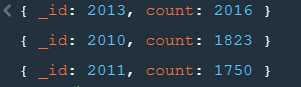
\includegraphics[width=0.6\textwidth]{query/mongo_q6.PNG}
\label{fig:query6}
\end{figure}

\subsection{Query 7}
This query returns the 20 most frequent \verb |keywords|.\newline
\textbf{Description:} the query starts by unwinding the keywords array. The next stage groups with respect to the
keywords (case insensitive) and computes the count for each group. Finally, the results are ordered by descending order
and limited to the top 20
\begin{lstlisting}
db.articles.aggregate([
	{$unwind: "$keywords" },
	{
		$group: {
			_id: {$toLower: '$keywords'},
			count: {$sum: 1}
		}
	},
	{$sort : { count : -1}},
	{$limit : 20}
]);
\end{lstlisting}
\begin{figure}[H]
\centering
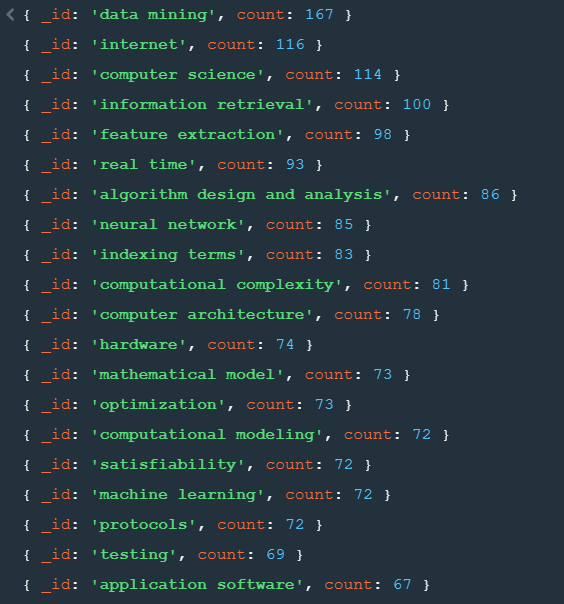
\includegraphics[width=0.5\textwidth]{query/mongo_q7.PNG}
\label{fig:query7}
\end{figure}

\subsection{Query 8}
This query, given the title of an article, returns the chapter with the highest number of images.\newline
\textbf{Description:} the first stage matches the article given the title. Then an unwind of the chapters array is
performed. The project stage is used to compute the variable \verb|imgCount| which stores the number of images
contained in each chapter. The results are sorted by descending order and limited to top 1.
\begin{lstlisting}
db.articles.aggregate([
	{"$match" : {title: "Locality Sensitive Outlier Detection: A ranking driven approach"}},
	{"$unwind" : {path: "$chapters"}},
	{"$project": {
		"title":1,
		"chapters":1,
		"imgCount": { "$size": "$chapters.images" } } },
	{"$sort": {imgCount:-1}},
	{"$limit": 1}
]);
\end{lstlisting}
\begin{figure}[H]
\centering
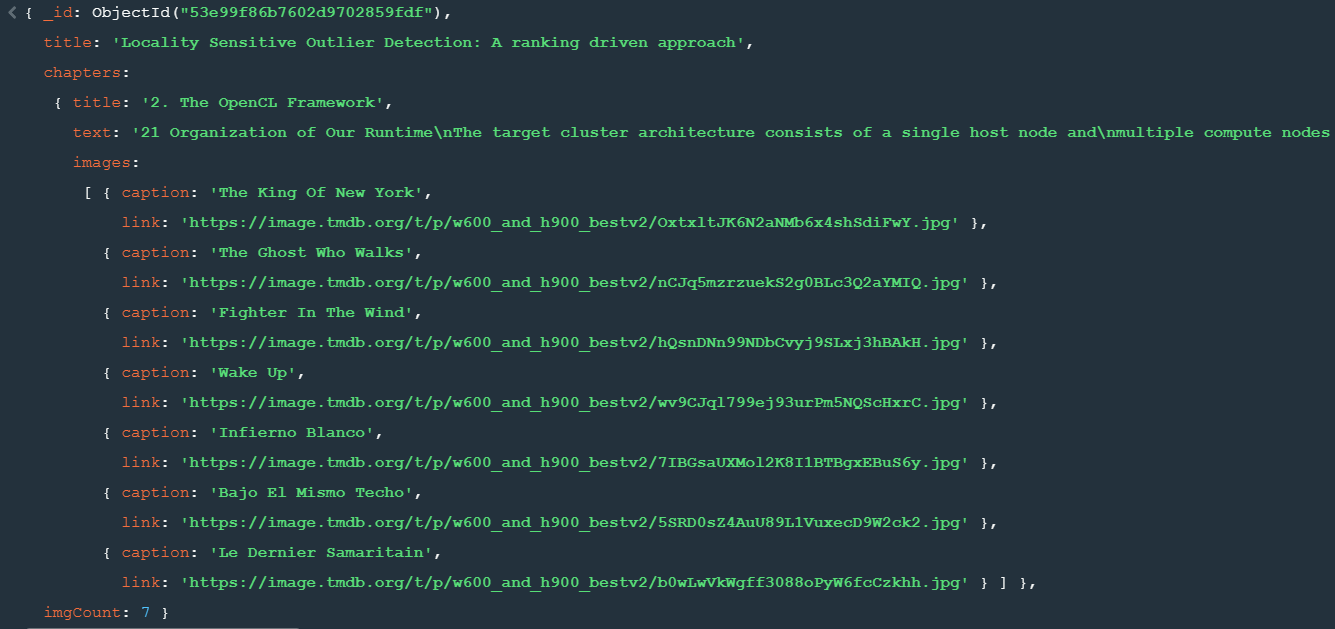
\includegraphics[width=1\textwidth]{query/mongo_q8.PNG}
\label{fig:query8}
\end{figure}

\subsection{Query 9}
This query returns articles citing another article that contains, between its \verb |references|, at least one
article written in a Milan University. \newline
\textbf{Description:} the first stage loads, by id, the array of cited documents into a new field called refs.
Then a match is used to find in this field all the articles that contain at least 1 author that worked for
a Milan university.\newline
\textbf{Note:} we used the operator \verb |lookup| to issue a join, in order to access another article instance.
\begin{lstlisting}
db.articles.aggregate([
	{$lookup: {
		from: "articles",
		localField: "references",
		foreignField: "_id",
		as: "refs"
		}
	},
	{$match: {
		"refs.authors.org":{$regex: "Milan"}
		}
	},
	{"$project": {
		"title":1,
		"refs.title":1,
		"refs.authors": 1
		}
	}
])
\end{lstlisting}
\begin{figure}[H]
\centering
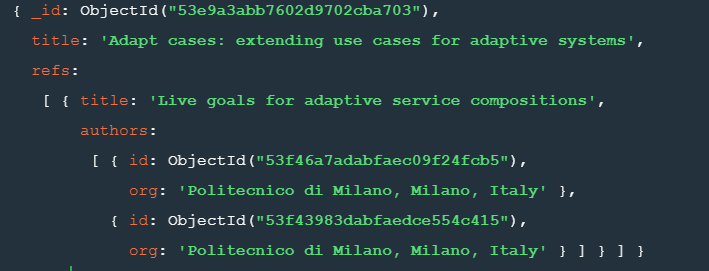
\includegraphics[width=0.9\textwidth]{query/mongo_q9.PNG}
\caption{Projection on title, refs.title, refs.authors}
\label{fig:query9}
\end{figure}

\subsection{Query 10}
This query finds the author with the maximum amount of written articles and retrieves his article with the highest number
of \verb |coauthors|.\newline
\textbf{Description:} First of all, we compute the \verb |artCount| field which contains the length of the articles array field.
Then we sort in descending order and keep only the first author by \verb |artCount|. After that, a join is performed to load the
articles documents into the new field \verb |articles_doc|. A new projection is then used to compute the number of authors of
each loaded article. Finally we sort the result in descending order and keep only the top 1 article. The projection is used
to display the result in a clearer way.\newline
\textbf{Note:} we used the operator \verb |lookup| to issue a join in order to access articles of the author.
\begin{lstlisting}
db.authors.aggregate([
	{"$project": {
		"_id":1,
		"name":1,
		"articles":1,
		"artCount": { "$size": "$articles" } } },
	{$sort : {"artCount": -1}},
	{$limit :1 },
	{$lookup: {
		from: "articles",
		localField: "articles",
		foreignField: "_id",
		as: "articles_doc"}},
	{"$project": {
		"name":1,
		"articles_doc":1,
		"authCount": { "$size": "$articles_doc.authors"}}},
	{$sort : { "authCount": -1}},
	{$limit : 1},
	{"$project": {
		"name":1,
		"articles_doc.title":1,
		"authCount": 1}}
])
\end{lstlisting}
\begin{figure}[H]
\centering
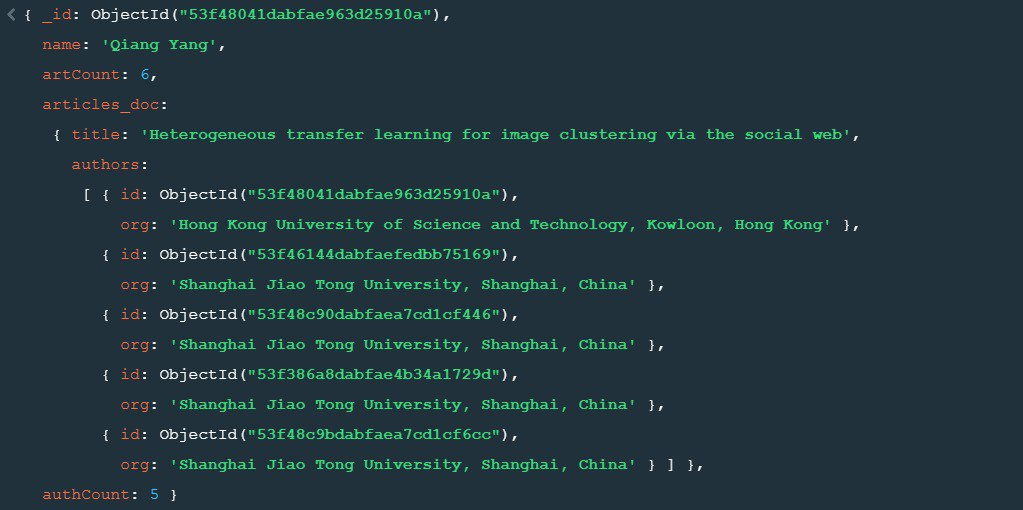
\includegraphics[width=1\textwidth]{query/mongo_q10.PNG}
\caption{Projection on name, articles\_doc.title, authCount}
\label{fig:query10}
\end{figure}

\subsection{Query 11}
This query returns all the articles written by authors whose names combined have all 26 letters of the alphabet.\newline
\textbf{Desciption:} The query is done with the following steps:
	\begin{itemize}
		\item an unwind on articles is performed to obtain an entry for each article written by an author
		\item results are sorted by authors' name in order to have the list sorted alphabetically for further steps
		\item for each article, a group is performed and the authors list is pushed into an array
		\item a string concatenating all the authors names retrieved by article documents, is computed and converted to lowercase
		\item a map operation is performed to split letter by letter the entries; a filter with a regex to keep only alphabet
			characters is applied, then an unwind on letters is made
		\item entries are then grouped by article \verb|_id| and authors list; letters are reduced into an array, then the
			size of this array is computed and only entries containing all 26 letters are matched
		\item finally, a join operation is performed on articles to obtain the title
	\end{itemize}
\begin{lstlisting}
db.authors.aggregate([
	{
		"$unwind" : {path: "$articles"}
	},
	{ "$sort" : { "name": 1 }},
	{
		"$group" : {
			_id: "$articles",
			authors: {
				$push: {
					$concat: ["$name"]
				}
			}
		},
	},
	{
		$project: {
			"_id": 1,
			"authors": "$authors",
			"fullNames": {
				$reduce: {
					input: "$authors",
					initialValue: "",
					in: { $toLower: {$concat : ["$$value", "$$this"]}}
				}
			}
		}
	},
	{
		$project: {
			"_id": 1,
			"authors": "$authors",
			letters: {
				$filter: {
					input: {
						$map: {
							input: {
								$range: [ 0, { "$strLenCP": "$fullNames" } ]
							},
							in: {
								"$substrCP":
								[
									"$fullNames",
									"$$this",
									1
								]
							}
						}
					},
					cond: {
						$regexMatch: {
							input: "$$this",
							regex: '[a-z]'
						}
					}
				}
			}
		}
	},
	{ $unwind: '$letters'},
	{
		$group: {
			_id: {
				"_id": '$_id',
				authors: "$authors"
			},
			letters: { $addToSet: '$letters' },
		}
	},
	{
		$project: {
			"_id" : 1,
			"authors": "$authors",
			"differentLetters": {
				"$size": "$letters"
			}
		}
	},
	{ $match : {"differentLetters" : 26}},
	{
		$lookup: {
			from: "articles",
			localField: "_id._id",
			foreignField: "_id",
			as: "articles_doc"
		}
	},
	{
		$project: {
			"_id": "$_id._id",
			"title": "$articles_doc.title",
			"authors": "$_id.authors",
			"differentLetters": "$differentLetters"
		}
	}
])
\end{lstlisting}
\begin{figure}[H]
\centering
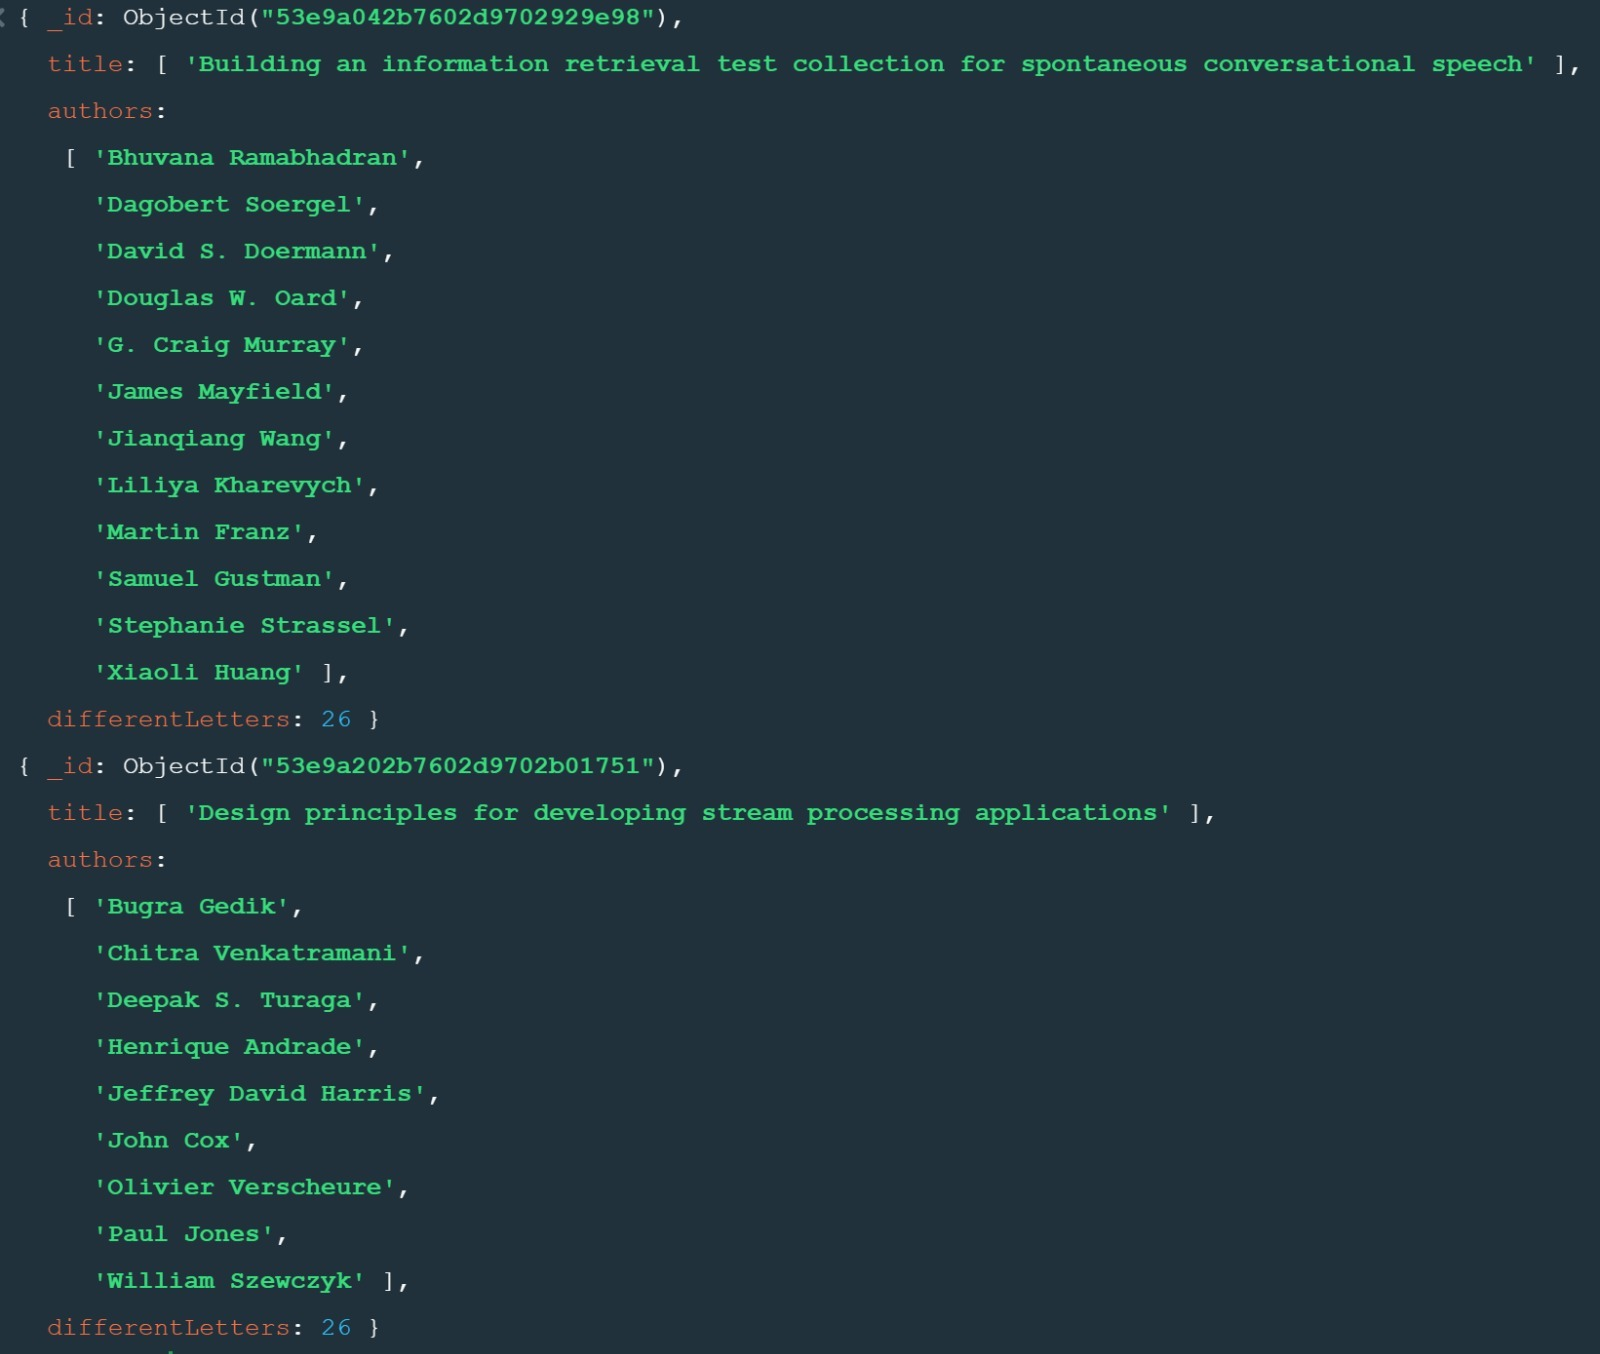
\includegraphics[width=1\textwidth]{query/mongo_q11.jpeg}
\caption{Projection on \_id, title, authors, differentLetters}
\label{fig:query11}
\end{figure}

\subsection{Improving Queries Perfomance}
In the queries, we performed string searches on relatively small textual fields using the \$regex operator.
This kind of search is easy to use and works very well on small datasets, but it is not optimal in large databases as it is not utilizing indexes efficiently.
If we wanted to perform advanced and high-performing full-text search queries, we would have had to define textual indexes among the two collections.
Since only one textual index can be created over a collection, an index over multiple textual fields should be defined.
These indexes can require some disk space and use a lot of resources when created.


\chapter{Conclusions}
The documental approach turned out to be very flexible and intuitive, thanks to its affinity with the object-oriented paradigm.
Also, this kind of technology allowed us to shape data to match the most frequent operations that could take place in the
publication domain. Therefore, queries became very simple and efficient.\newline
Moreover, with our implementation, we tried to reach a good trade-off between performance and spatial complexity, avoiding
choices that could lead to critical data duplication problems.


\end{document}
